%
%  untitled
%
%  Created by Parham Aram on 2010-07-14.
%  Copyright (c) 2010 . All rights reserved.
%
\documentclass[]{article}

% Setup for fullpage use
\usepackage{fullpage}

\usepackage[pdftex]{graphicx}


% More symbols
\usepackage{amsmath}
\usepackage{amssymb}

\usepackage[usenames,dvipsnames]{color}
\newcommand{\dean}[1]{\textcolor{red}{#1}}
\newcommand{\parham}[1]{\textcolor{blue}{#1}}

\begin{document}


\renewcommand{\theequation}{S1.\arabic{equation}}


\subsection*{Estimation of Connectivity Kernel Support}
The support of the connectivity kernel can be inferred using spatial correlation analysis. The method presented in this paper is based on a similar published method, where the kernel support was estimated using correlation analysis for a linear system described by an IDE~\cite{Scerri2009}. To demonstrate the method for the neural field model we assume the sensors are infinitesimally close (continuous observation). The spatial cross-correlation function between consecutive observations is defined as 
\begin{align}
	R_{y_{t},y_{t+1}}(\boldsymbol{\tau}) &= \mathbf{E}\left[ y_{t}\left(\mathbf{r}\right) y_{t+1}\left(\mathbf{r}+\boldsymbol{\tau}\right) \right] \\
	&= \mathbf{E}\left[\left(m\left(\mathbf{r}\right) \ast v_t\left(\mathbf{r}\right) + \boldsymbol{\varepsilon}_t\left(\mathbf{r}\right) \right) \times \left( m\left(\mathbf{r}+\boldsymbol{\tau}\right) \ast v_{t+1}\left(\mathbf{r}+\boldsymbol{\tau}\right) + \boldsymbol{\varepsilon}_{t+1}\left(\mathbf{r}+\boldsymbol{\tau}\right)\right) \right], \label{eq:ObsXCorr}
\end{align}
where $\mathbf{E}[\cdot]$ is the expected value. Since the observation noise is zero mean, temporally white and independent of the field, equation~\ref{eq:ObsXCorr} reduces to
\begin{equation}
	R_{y_{t},y_{t+1}}(\boldsymbol{\tau}) = \mathbf{E}\left[ m\left(\mathbf{r}\right) \ast v_t\left(\mathbf{r}\right) \times m\left(\mathbf{r}+\boldsymbol{\tau}\right) \ast v_{t+1}\left(\mathbf{r}+\boldsymbol{\tau}\right) \right].
\end{equation}
Substituting in equation~\ref{DiscreteTimeModel}  for $v_{t+1}\left(\mathbf{r}\right)$, the cross-correlation function is
\begin{align}
	R_{y_{t},y_{t+1}}(\boldsymbol{\tau}) &= \mathbf{E}\left[ m\left(\mathbf{r}\right) \ast v_t\left(\mathbf{r}\right) \times m\left(\mathbf{r}+\boldsymbol{\tau}\right) \ast \left( \xi v_t\left(\mathbf{r}+\boldsymbol{\tau}\right) + T_s w\left(\mathbf{r}+\boldsymbol{\tau}\right) \ast f\left(v_t\left(\mathbf{r}+\boldsymbol{\tau}\right)\right) + e_t\left(\mathbf{r}+\boldsymbol{\tau}\right)\right) \right] \\	
	 &= \xi \mathbf{E}\left[ m\left(\mathbf{r}\right) \ast v_t\left(\mathbf{r}\right) \times m\left(\mathbf{r}+\boldsymbol{\tau}\right) \ast v_t\left(\mathbf{r}+\boldsymbol{\tau}\right) \right] \nonumber \\
	&+ T_s\mathbf{E}\left[ m\left(\mathbf{r}\right) \ast v_t\left(\mathbf{r}\right) \times m\left(\mathbf{r}+\boldsymbol{\tau}\right) \ast w\left(\mathbf{r}+\boldsymbol{\tau}\right) \ast f\left(v_t\left(\mathbf{r}+\boldsymbol{\tau}\right)\right) \right] \nonumber \\
	&+ \mathbf{E}\left[ m\left(\mathbf{r}\right) \ast v_t\left(\mathbf{r}\right) \times m\left(\mathbf{r}+\boldsymbol{\tau}\right) \ast e_t\left(\mathbf{r}+\boldsymbol{\tau}\right) \right]
	\\
	&= R_1(\boldsymbol{\tau}) + R_2(\boldsymbol{\tau}) + R_3(\boldsymbol{\tau}).\label{eq:spatialxcorr} 
\end{align}
The first term, $R_1(\boldsymbol{\tau})$, can be simplified to
\begin{align}
	R_1(\boldsymbol{\tau}) &= \xi \mathbf{E}\left[ m\left(\mathbf{r}\right) \ast v_t\left(\mathbf{r}\right) \times m\left(\mathbf{r}+\boldsymbol{\tau}\right) \ast v_t\left(\mathbf{r}+\boldsymbol{\tau}\right) \right] \\
	&= \xi\left( R_{y_{t},y_{t}}(\boldsymbol{\tau}) - \sigma_{\varepsilon}\delta_K\left(\boldsymbol{\tau}\right) \right). \label{eq:R1}
\end{align}
The second term
\begin{equation}
	R_2(\boldsymbol{\tau}) = T_s\mathbf{E}\left[ m\left(\mathbf{r}\right) \ast v_t\left(\mathbf{r}\right) \times m\left(\mathbf{r}+\boldsymbol{\tau}\right) \ast w\left(\mathbf{r}+\boldsymbol{\tau}\right) \ast f\left(v_t\left(\mathbf{r}+\boldsymbol{\tau}\right)\right) \right]
\end{equation}
Now we assume that the sigmoid activation function, $f(\cdot)$, can be approximated by the piecewise function
\begin{equation}
	\hat{f}(v_t(\mathbf{r}')) = \left\{ \begin{array}{ll}
		0, & v_t(\mathbf{r}') \le v_1 \\
		\varsigma v_t(\mathbf{r}'), &  v_1 < v_t(\mathbf{r}') < v_2 \\
		1, & v_t(\mathbf{r}') \ge v_2 \\ 
		\end{array}\right.
\end{equation}
Furthermore, we assume the field is in the linear region of the piecewise function for the majority of the time giving
\begin{equation}
	R_2(\boldsymbol{\tau}) \approx T_s\mathbf{E}\left[ m\left(\mathbf{r}\right) \ast v_t\left(\mathbf{r}\right) \times m\left(\mathbf{r}+\boldsymbol{\tau}\right) \ast w\left(\mathbf{r}+\boldsymbol{\tau}\right) \ast \varsigma v_t\left(\mathbf{r}+\boldsymbol{\tau}\right) \right].
\end{equation}
$R_2(\boldsymbol{\tau})$ can be written as
\begin{align}
	R_2(\boldsymbol{\tau}) &\approx	T_s \varsigma \mathbf{E}\left[ \hat{y}\left(\mathbf{r}\right) \times \hat{y}\left(\mathbf{r}+\boldsymbol{\tau}\right) \ast w\left(\mathbf{r}+\boldsymbol{\tau}\right)\right] \\
	&= T_s \varsigma \mathbf{E}\left[ \hat{y}\left(\mathbf{r}\right)  \int_{\Omega}\hat{y}\left(\mathbf{r'}\right) w\left(\mathbf{r}+\boldsymbol{\tau}-\mathbf{r'}\right) d\mathbf{r'} \right] \\
	&= T_s \varsigma \mathbf{E}\left[  \int_{\Omega}\hat{y}\left(\mathbf{r}\right)\hat{y}\left(\mathbf{r'}\right) w\left(\mathbf{r}+\boldsymbol{\tau}-\mathbf{r'}\right) d\mathbf{r'} \right] \\
	&= T_s \varsigma \mathbf{E}\left[  \int_{\Omega}\hat{y}\left(\mathbf{r}\right)\hat{y}\left(\mathbf{r'}+\mathbf{r}\right) w\left(\boldsymbol{\tau}-\mathbf{r'}\right) d\mathbf{r'} \right] \\
	&= T_s \varsigma   \int_{\Omega}\mathbf{E}\left[\hat{y}\left(\mathbf{r}\right)\hat{y}\left(\mathbf{r'}+\mathbf{r}\right) \right] w\left(\boldsymbol{\tau}-\mathbf{r}'\right) d\mathbf{r'} \nonumber \\
	&=T_s \varsigma  \int_{\Omega} R_1(\mathbf{r'}) w\left(\boldsymbol{\tau}-\mathbf{r}'\right) d\mathbf{r'} \nonumber \\
	&=T_s \varsigma \left(R_1 \ast w\right)\left(\boldsymbol{\tau}\right)\\
\end{align}
This can be simplified to
\begin{align}
	R_2(\boldsymbol{\tau}) &\approx T_s \varsigma \left( R_{y_{t},y_{t}}(\boldsymbol{\tau}) - \sigma_{\varepsilon}^2 \delta_K\left(\boldsymbol{\tau}\right) \right) \ast w\left(\boldsymbol{\tau}\right) \\
	&= \frac{T_s \varsigma}{\xi} R_1(\boldsymbol{\tau}) \ast w\left(\boldsymbol{\tau}\right)
\end{align}
The last term on the right hand side of equation~\ref{eq:spatialxcorr} is
\begin{equation}
	R_3(\boldsymbol{\tau}) = 0,
\end{equation}
since the disturbance added to the field at time $t$ and assumed to be uncorrelated to the field at time $t$. Therefore 
\begin{equation}
	R_{y_{t},y_{t+1}}(\boldsymbol{\tau}) - R_1(\boldsymbol{\tau}) \approx \frac{T_s \varsigma}{\xi} R_1(\boldsymbol{\tau}) \ast w\left(\boldsymbol{\tau}\right).
\end{equation}
Now, by taking the Fourier transform we get
\begin{equation}
	\mathcal{F}\left\{R_{y_{t},y_{t+1}}(\boldsymbol{\tau})\right\} - \mathcal{F}\left\{R_1(\boldsymbol{\tau})\right\} \approx \frac{T_s \varsigma}{\xi} \mathcal{F}\left\{R_1(\boldsymbol{\tau})\right\} \mathcal{F}\left\{ w\left(\boldsymbol{\tau}\right)\right\}.
\end{equation}
This simplifies to
\begin{equation}
	\frac{\xi}{T_s \varsigma} \left(\frac{\mathcal{F}\left\{R_{y_{t},y_{t+1}}(\boldsymbol{\tau})\right\}}{\mathcal{F}\left\{R_1(\boldsymbol{\tau})\right\}} - 1\right) \approx  \mathcal{F}\left\{ w\left(\boldsymbol{\tau}\right)\right\}.
\end{equation}
Now substituting back in equation~\ref{eq:R1}, we can write

\begin{align}
	\mathcal{F}\left\{ w\left(\boldsymbol{\tau}\right)\right\} &\approx \frac{\xi}{T_s \varsigma} \left(\frac{\mathcal{F}\left\{R_{y_{t},y_{t+1}}(\boldsymbol{\tau})\right\}}{\mathcal{F}\left\{\xi\left( R_{y_{t},y_{t}}(\boldsymbol{\tau}) - \sigma_{\varepsilon}^2\delta_K\left(\boldsymbol{\tau}\right) \right)\right\}} - 1\right)  \\
	&= \frac{1}{T_s \varsigma} \left(\frac{\mathcal{F}\left\{R_{y_{t},y_{t+1}}(\boldsymbol{\tau})\right\}}{\mathcal{F}\left\{ R_{y_{t},y_{t}}(\boldsymbol{\tau})\right\} - \sigma_{\varepsilon}^2 } - \xi\right) \\
	&= \frac{1}{T_s \varsigma} \left(\frac{S_{y_{t},y_{t+1}}\left(\boldsymbol{\nu}\right)}{S_{y_{t},y_{t}}\left(\boldsymbol{\nu}\right) - \sigma_{\varepsilon}^2 } - \xi\right)
\end{align}

% Putting to other two terms back together we can write
% \begin{equation}
% 	R_{y_{t},y_{t+1}}(\boldsymbol{\tau}) = \mathbf{E}\left[ m\left(\mathbf{r}\right) \ast v_t\left(\mathbf{r}\right) \times m\left(\mathbf{r}+\boldsymbol{\tau}\right) \ast \left(\xi v_t\left(\mathbf{r}+\boldsymbol{\tau}\right) + T_s w\left(\mathbf{r}+\boldsymbol{\tau}\right) \ast f\left(v_t\left(\mathbf{r}+\boldsymbol{\tau}\right)\right) \right) \right]
% \end{equation}
% Now we assume that the sigmoid activation function, $f(\cdot)$, can be approximated by the piecewise function
% \begin{equation}
% 	\hat{f}(v_t(\mathbf{r}')) = \left\{ \begin{array}{ll}
% 		0, & v_t(\mathbf{r}') \le v_1 \\
% 		\varsigma v_t(\mathbf{r}'), &  v_1 < v_t(\mathbf{r}') < v_2 \\
% 		1, & v_t(\mathbf{r}') \ge v_2 \\ 
% 		\end{array}\right.
% \end{equation}
% Furthermore, we assume the field is in the linear region of the piecewise function for the majority of the time. 
% \begin{equation}
% 	R_{y_{t},y_{t+1}}(\boldsymbol{\tau}) \approx \mathbf{E}\left[ m\left(\mathbf{r}\right) \ast v_t\left(\mathbf{r}\right) \times m\left(\mathbf{r}+\boldsymbol{\tau}\right) \ast \left(\xi v_t\left(\mathbf{r}+\boldsymbol{\tau}\right) + T_s w\left(\mathbf{r}+\boldsymbol{\tau}\right) \ast \varsigma v_t\left(\mathbf{r}+\boldsymbol{\tau}\right) \right) \right]
% \end{equation}
% Now we take the Fourier transform of the terms inside the expectation giving
% \begin{align}
% 	R_{y_{t},y_{t+1}}(\boldsymbol{\tau}) &\approx \mathbf{E}\left[\mathcal{F}^{-1} \left\{M(\boldsymbol{\nu})V(\boldsymbol{\nu}) \ast \left(\xi e^{i\boldsymbol{\nu}^{\top}\boldsymbol{\tau}} M(\boldsymbol{\nu}) e^{i\boldsymbol{\nu}^{\top}\boldsymbol{\tau}} V(\boldsymbol{\nu}) + T_s e^{i\boldsymbol{\nu}^{\top}\boldsymbol{\tau}} M(\boldsymbol{\nu}) e^{i\boldsymbol{\nu}^{\top}\boldsymbol{\tau}} W(\boldsymbol{\nu}) e^{i\boldsymbol{\nu}^{\top}\boldsymbol{\tau}} \varsigma V(\boldsymbol{\nu}) \right) \right\} \right] \\
% 	&= \mathbf{E}\left[\mathcal{F}^{-1} \left\{M(\boldsymbol{\nu}) V(\boldsymbol{\nu}) \ast \left(\xi e^{2i\boldsymbol{\nu}^{\top}\boldsymbol{\tau}} M(\boldsymbol{\nu}) V(\boldsymbol{\nu}) + T_s \varsigma e^{2i\boldsymbol{\nu}^{\top}\boldsymbol{\tau}} M(\boldsymbol{\nu})  V(\boldsymbol{\nu}) e^{i\boldsymbol{\nu}^{\top}\boldsymbol{\tau}} W(\boldsymbol{\nu}) \right) \right\} \right]
% \end{align}
% Expand brackets
% \begin{equation}
% 	R_{y_{t},y_{t+1}}(\boldsymbol{\tau}) \approx \mathbf{E}\left[\mathcal{F}^{-1} \left\{M(\boldsymbol{\nu}) V(\boldsymbol{\nu}) \ast  \xi e^{2i\boldsymbol{\nu}^{\top}\boldsymbol{\tau}} M(\boldsymbol{\nu}) V(\boldsymbol{\nu}) + M(\boldsymbol{\nu}) V(\boldsymbol{\nu}) \ast T_s \varsigma e^{2i\boldsymbol{\nu}^{\top}\boldsymbol{\tau}} M(\boldsymbol{\nu}) V(\boldsymbol{\nu}) e^{i\boldsymbol{\nu}^{\top}\boldsymbol{\tau}} W(\boldsymbol{\nu}) \right\} \right]
% \end{equation}
% 
% Now taking the inverse Fourier transform we get
% \begin{equation}
% 	R_{y_{t},y_{t+1}}(\boldsymbol{\tau}) \approx \mathbf{E}\left[m(\mathbf{r}) \ast v_t(\mathbf{r}) \times \xi m(\mathbf{r}+\boldsymbol{\tau}) \ast v_t(\mathbf{r}+\boldsymbol{\tau}) +  m(\mathbf{r}) \ast v_t(\mathbf{r}) \times T_s \varsigma m(\mathbf{r}+\boldsymbol{\tau}) \ast v_t(\mathbf{r}+\boldsymbol{\tau}) \ast w(\mathbf{r}+\boldsymbol{\tau}) \right]
% \end{equation}
% Split the expectation at the plus sign
% \begin{align}
% 	R_{y_{t},y_{t+1}}(\boldsymbol{\tau}) &\approx \xi \mathbf{E}\left[m(\mathbf{r}) \ast v_t(\mathbf{r}) \times  m(\mathbf{r}+\boldsymbol{\tau}) \ast v_t(\mathbf{r}+\boldsymbol{\tau}) \right] \\
% 	&+ T_s \varsigma \mathbf{E}\left[  m(\mathbf{r}) \ast v_t(\mathbf{r}) \times  m(\mathbf{r}+\boldsymbol{\tau}) \ast v_t(\mathbf{r}+\boldsymbol{\tau}) \ast w(\mathbf{r}+\boldsymbol{\tau}) \right] \\
% 	&= \xi \left(R_{y_{t},y_{t}}(\boldsymbol{\tau}) - \sigma_{\varepsilon}\delta_K\left(\boldsymbol{\tau}\right)\right) \\
% 	&+ T_s \varsigma \mathbf{E}\left[  m(\mathbf{r}) \ast v_t(\mathbf{r}) \times  m(\mathbf{r}+\boldsymbol{\tau}) \ast v_t(\mathbf{r}+\boldsymbol{\tau}) \right]  \ast w(\boldsymbol{\tau}) \\
% 	&= \xi \left( R_{y_{t},y_{t}}(\boldsymbol{\tau}) - \sigma_{\varepsilon}\delta_K\left(\boldsymbol{\tau}\right) \right) \\
% 	&+ T_s \varsigma \left( R_{y_{t},y_{t}}(\boldsymbol{\tau}) - \sigma_{\varepsilon}\delta_K\left(\boldsymbol{\tau}\right) \right) \ast w(\boldsymbol{\tau})
% \end{align}
% 
% Now rearrange to get
% \begin{align}
% 	R_{y_{t},y_{t+1}}(\boldsymbol{\tau}) - \xi \left( R_{y_{t},y_{t}}(\boldsymbol{\tau}) - \sigma_{\varepsilon}\delta_K\left(\boldsymbol{\tau}\right) \right) \approx T_s \varsigma \left( R_{y_{t},y_{t}}(\boldsymbol{\tau}) - \sigma_{\varepsilon}\delta_K\left(\boldsymbol{\tau}\right) \right) \ast w(\boldsymbol{\tau})
% \end{align}
% 
% Taking the Fourier transform gives
% \begin{equation}
% 	\frac{1}{T_s \varsigma}\mathcal{F}^{-1}\left\{\frac{\mathcal{F}\left\{ R_{y_{t},y_{t+1}}(\boldsymbol{\tau}) - \xi \left( R_{y_{t},y_{t}}(\boldsymbol{\tau}) - \sigma^2_{\varepsilon}\delta_K\left(\boldsymbol{\tau}\right) \right) \right\}} {  \mathcal{F} \left\{  R_{y_{t},y_{t}}(\boldsymbol{\tau}) - \sigma^2_{\varepsilon}\delta_K\left(\boldsymbol{\tau}\right) \right\}}\right\} \approx  w(\boldsymbol{\tau})	
% \end{equation}
% Simplify
% \begin{equation}
% 	\frac{1}{T_s \varsigma}\mathcal{F}^{-1}\left\{\frac{(1 - \xi)\mathcal{F}\left\{ R_{y_{t},y_{t+1}}(\boldsymbol{\tau}) \right\} - \xi \sigma^2_{\varepsilon} } {  \mathcal{F} \left\{  R_{y_{t},y_{t}}(\boldsymbol{\tau}) \right\} - \sigma^2_{\varepsilon} }\right\} \approx  w(\boldsymbol{\tau})	
% \end{equation}
% 
% \begin{align}
% 	R_{y_{t},y_{t+1}}(\boldsymbol{\tau}) &\approx \mathbf{E}\left[m(\mathbf{r}) \ast v_t(\mathbf{r}) \times \left( m(\mathbf{r}+\boldsymbol{\tau}) \ast v_t(\mathbf{r}+\boldsymbol{\tau}) \ast \xi\delta_D(\mathbf{r}) + T_s \varsigma m(\mathbf{r}+\boldsymbol{\tau}) \ast v_t(\mathbf{r}+\boldsymbol{\tau}) \ast  w(\mathbf{r}+\boldsymbol{\tau})\right) \right] \\
% 	&= \mathbf{E}\left[m(\mathbf{r}) \ast v_t(\mathbf{r}) \times \left( m(\mathbf{r}+\boldsymbol{\tau}) \ast \xi v_t(\mathbf{r}+\boldsymbol{\tau}) + T_s \varsigma m(\mathbf{r}+\boldsymbol{\tau}) \ast v_t(\mathbf{r}+\boldsymbol{\tau}) \ast  w(\mathbf{r}+\boldsymbol{\tau})\right) \right] \\
% 	&= \mathbf{E}\left[m(\mathbf{r}) \ast v_t(\mathbf{r}) \times  m(\mathbf{r}+\boldsymbol{\tau}) \ast \xi v_t(\mathbf{r}+\boldsymbol{\tau}) + m(\mathbf{r}) \ast v_t(\mathbf{r}) \times T_s \varsigma m(\mathbf{r}+\boldsymbol{\tau}) \ast v_t(\mathbf{r}+\boldsymbol{\tau}) \ast  w(\mathbf{r}+\boldsymbol{\tau}) \right] \\
% 	&= \mathbf{E}\left[m(\mathbf{r}) \ast v_t(\mathbf{r}) \times  m(\mathbf{r}+\boldsymbol{\tau}) \ast \xi v_t(\mathbf{r}+\boldsymbol{\tau}) \right] + \mathbf{E}\left[ m(\mathbf{r}) \ast v_t(\mathbf{r}) \times T_s \varsigma m(\mathbf{r}+\boldsymbol{\tau}) \ast v_t(\mathbf{r}+\boldsymbol{\tau}) \ast  w(\mathbf{r}+\boldsymbol{\tau}) \right] \\
% 	&= R_{y_{t},y_{t}}(\boldsymbol{\tau}) - \sigma_{\varepsilon}\delta_K\left(\boldsymbol{\tau}\right) + \mathbf{E}\left[ m(\mathbf{r}) \ast v_t(\mathbf{r}) \times T_s \varsigma m(\mathbf{r}+\boldsymbol{\tau}) \ast v_t(\mathbf{r}+\boldsymbol{\tau}) \ast  w(\mathbf{r}+\boldsymbol{\tau}) \right] \\
% 	&= R_{y_{t},y_{t}}(\boldsymbol{\tau}) - \sigma_{\varepsilon}\delta_K\left(\boldsymbol{\tau}\right) + \mathbf{E}\left[ m(\mathbf{r}) \ast v_t(\mathbf{r}) \times  m(\mathbf{r}+\boldsymbol{\tau}) \ast v_t(\mathbf{r}+\boldsymbol{\tau})\right] \ast T_s \varsigma w(\boldsymbol{\tau}) \\
% 	% 	&\parham{= \mathbf{E}\left[m(\mathbf{r}) \ast v_t(\mathbf{r}) \times m(\mathbf{r}+\boldsymbol{\tau}) \ast v_t(\mathbf{r}+\boldsymbol{\tau}) \right] \ast \mathbf{E}\left[\left( \xi\delta_D(\mathbf{r}) + T_s \varsigma w(\mathbf{r}+\boldsymbol{\tau}) \right) \right]} \label{eq:xcorr_pre_sub}
% \end{align}
% \parham{From (S1.14) to (S1.15) doesn't hold.} where $\mathcal{F}^{-1}$ denotes the inverse Fourier transform and $R_{y_{t},y_{t}}(\boldsymbol{\tau})$ is the auto-correlation of the observations, $\delta_K(\cdot)$ is the Kronecker delta function, and $\delta_D(\cdot)$ is the Dirac delta function. We define the auto-correlation of the observations as
% \begin{align}
% 	R_{y_{t},y_{t}}(\boldsymbol{\tau}) &= \mathbf{E}\left[ y_{t}\left(\mathbf{r}\right) y_{t}\left(\mathbf{r}+\boldsymbol{\tau}\right) \right]\\
% 	&= \mathbf{E}\left[m(\mathbf{r}) \ast v_t(\mathbf{r}) \times m(\mathbf{r}+\boldsymbol{\tau}) \ast v_t(\mathbf{r}+\boldsymbol{\tau})\right] + \delta_K(\boldsymbol{\tau})\sigma_{\varepsilon}^2
% \end{align}
% Rearrange to get
% \begin{equation}\label{eq:autocorr_for_sub}
% 	R_{y_{t},y_{t}}(\boldsymbol{\tau}) - \delta_K(\boldsymbol{\tau})\sigma_{\varepsilon}^2 = \mathbf{E}\left[m(\mathbf{r}) \ast v_t(\mathbf{r}) \times m(\mathbf{r}+\boldsymbol{\tau}) \ast v_t(\mathbf{r}+\boldsymbol{\tau})\right].
% \end{equation}
% Now to isolate the kernel equation~\ref{eq:autocorr_for_sub} is substituted into equation~\ref{eq:xcorr_pre_sub} and the Fourier transform is taken giving
% \begin{align}
% 	\mathcal{F}\left\{R_{y_{t},y_{t+1}}(\boldsymbol{\tau})\right\} &\approx \mathcal{F}\left\{ \left(R_{y_t,y_t}(\boldsymbol{\tau}) - \delta_K\left(\boldsymbol{\tau}\right)\sigma_{\varepsilon}^2\right) \ast \mathbf{E} \left[ \xi\delta_D(\mathbf{r})  + T_s \varsigma w(\mathbf{r}+\boldsymbol{\tau}) \right] \right\} \\
% 	&= \mathcal{F}\left\{ R_{y_t,y_t}(\boldsymbol{\tau}) - \delta_K\left(\boldsymbol{\tau}\right) \sigma_{\varepsilon}^2 \right\} \mathcal{F}\left\{\mathbf{E}[ \xi \delta_D(\mathbf{r})  + T_s \varsigma w(\mathbf{r}+\boldsymbol{\tau}) ]\right\}.
% \end{align}
% Now rearranging
% \begin{equation}
% 	\frac{\mathcal{F}\left\{R_{y_{t},y_{t+1}}(\boldsymbol{\tau})\right\}}{\mathcal{F}\left\{ R_{y_t,y_t}(\boldsymbol{\tau}) - \delta_K\left(\boldsymbol{\tau}\right)\sigma_{\varepsilon}^2 \right\}} \approx \mathcal{F}\left\{ \mathbf{E}\left[ \xi\delta_D\left(\mathbf{r}\right)  + T_s \varsigma w(\mathbf{r}+\boldsymbol{\tau}) \right]\right\}.
% \end{equation}
% Take inverse Fourier transform and rearrange to get an approximation of the kernel
% \begin{equation}
% 	\mathcal{F}^{-1}\left\{\frac{\mathcal{F}\left\{R_{y_{t},y_{t+1}}(\boldsymbol{\tau})\right\}}{\mathcal{F}\left\{ R_{y_t,y_t}(\boldsymbol{\tau}) - \delta_K\left(\boldsymbol{\tau}\right)\sigma_{\varepsilon}^2 \right\}}\right\} \approx \mathbf{E}[\xi\delta_D\left(\mathbf{r}\right)  + T_s \varsigma w(\mathbf{r}+\boldsymbol{\tau})].
% \end{equation}
 This equation states that the support of the kernel can be estimated given knowledge of $\sigma_\varepsilon^2$. Furthermore, is we assume a local coupling (at $\boldsymbol\tau=0$) regime, either excitation or inhibition, than we don't even need to know $\sigma_\varepsilon^2$. The peak in the kernel at $\mathbf{r}=0$ will be bigger or smaller if we guess incorrectly and the kernel parameters can do the rest! 

\newpage
\section*{Observation Autocorrelation}\label{sec:ObservAutocor} 
\begin{align}
	R_{y_{t},y_{t}}(\boldsymbol{\tau}) &= \mathbf{E}\left[y_{t}\left(\mathbf{r}+\boldsymbol{\tau}\right)y_{t}\left(\mathbf{r}\right)\right] \nonumber\\
	&= \mathbf{E}\left[\left(\int_{\Omega}{ m\left(\mathbf{r} + \boldsymbol{\tau} - \mathbf{r}'\right) v_t\left(\mathbf{r}'\right)\, d\mathbf{r}'} + \boldsymbol{\varepsilon}_t\left(\mathbf{r}+\boldsymbol{\tau}\right)\right) \left(\int_{\Omega}{ m\left(\mathbf{r} - \mathbf{r}''\right) v_{t}\left(\mathbf{r}''\right) \, d\mathbf{r}''} + \boldsymbol{\varepsilon}_{t}\left(\mathbf{r}\right)\right) \right]\nonumber \\
	&=\mathbf{E}\left[\int_{\Omega}{ m\left(\mathbf{r} + \boldsymbol{\tau} - \mathbf{r}'\right) v_t\left(\mathbf{r}'\right)\, d\mathbf{r}'} \int_{\Omega}{ m\left(\mathbf{r} - \mathbf{r}''\right) v_{t}\left(\mathbf{r}''\right) \, d\mathbf{r}''}\right]+\sigma_{\epsilon}^2\delta(\boldsymbol\tau)\nonumber\\
	&=\iint_{\Omega}{ m\left(\mathbf{r} + \boldsymbol{\tau} - \mathbf{r}'\right) m\left(\mathbf{r} - \mathbf{r}''\right) \mathbf{E}\left[v_t\left(\mathbf{r}'\right) v_{t}\left(\mathbf{r}''\right)\right]\, d\mathbf{r}'}{ \, d\mathbf{r}''}+\sigma_{\epsilon}^2\delta(\boldsymbol\tau) \nonumber\\
	&=\sigma_d\iint_{\Omega}{ m\left(\mathbf{r} + \boldsymbol{\tau} - \mathbf{r}'\right) m\left(\mathbf{r} - \mathbf{r}''\right)\gamma(\mathbf{r}'-\mathbf{r}'') \, d\mathbf{r}'}{ \, d\mathbf{r}''}+\sigma_{\epsilon}^2\delta(\boldsymbol\tau)\nonumber \\
	&=\sigma_d\int_{\Omega} m\left(\mathbf r  + \boldsymbol\tau - \mathbf r'\right) \left[\int_{\Omega} m\left(\mathbf r - \mathbf r''\right)\gamma(\mathbf r'-\mathbf r'') \, d\mathbf r'' \right]  d\mathbf r'+\sigma_{\epsilon}^2\delta(\boldsymbol\tau)\label{eq:ObsCorr1}
\end{align}
the term in the bracket can be written
\begin{align}
 \int_{\Omega} m\left(\mathbf r - \mathbf r''\right)\gamma(\mathbf r'-\mathbf r'') \, d\mathbf r''&=\int_{\Omega} m\left(\mathbf r'' - \mathbf r\right)\gamma(\mathbf r'-\mathbf r'') \, d\mathbf r'' \nonumber \\
&=\int_{\Omega} m\left(\mathbf s\right)\gamma(\mathbf r'-\mathbf r-\mathbf s) \, d\mathbf s\nonumber \\
&=\left(m\ast\gamma\right)(\mathbf r'-\mathbf r)\label{eq:ObsCorr1term1}
\end{align}
where $\mathbf s=\mathbf r''-\mathbf r$ and therefore $d\mathbf r''=d\mathbf s$. Note that  $m\left(\mathbf{r}-\mathbf{r''}\right)=m\left(\mathbf{r''}-\mathbf{r}\right)$ due to the  symmetry of the observation kernel.
substituting \eqref{eq:ObsCorr1term1} in \eqref{eq:ObsCorr1} we have

\begin{align}
&\sigma_d\int_{\Omega} m\left(\mathbf r  + \boldsymbol\tau - \mathbf r'\right) \left[\int_{\Omega} m\left(\mathbf r - \mathbf r''\right)\gamma(\mathbf r'-\mathbf r'') \, d\mathbf r'' \right]  d\mathbf r'+\sigma_{\epsilon}^2\delta(\boldsymbol\tau) \nonumber \\
&=\sigma_d\int_{\Omega} m\left(\mathbf r  + \boldsymbol\tau - \mathbf r'\right) \left(m\ast\gamma\right)(\mathbf r'-\mathbf r) \ d\mathbf r'+\sigma_{\epsilon}^2\delta(\boldsymbol\tau)\\
&=\sigma_d\int_{\Omega} m\left(\boldsymbol\tau - \mathbf u\right) \left(m\ast\gamma\right)(\mathbf u) \ d\mathbf u+\sigma_{\epsilon}^2\delta(\boldsymbol\tau) \nonumber \\
&=\sigma_d\left(m \ast m \ast \gamma\right)\left(\boldsymbol{\tau}\right)+\sigma_{\epsilon}^2\delta(\boldsymbol\tau)
\end{align}
Therefore we have
\begin{align}
	R_{y_{t},y_{t}}(\boldsymbol{\tau}) &= \sigma_d\left(m \ast m \ast \gamma\right)\left(\boldsymbol{\tau}\right)+\sigma_{\epsilon}^2\delta(\boldsymbol\tau)\label{eq:ObservationAutocorrelation}
\end{align}
% \section*{Observation Crosscorrelation}\label{sec:ObservCroocor} 
% \begin{align}
% 	R_{y_{t},y_{t+1}}(\boldsymbol{\tau}) &= \mathbf{E}\left[y_{t}\left(\mathbf{r}+\boldsymbol{\tau}\right)y_{t+1}\left(\mathbf{r}\right)\right] \nonumber\\
% 	&= \mathbf{E}\left[\left(\int_{\Omega}{ m\left(\mathbf{r} + \boldsymbol{\tau} - \mathbf{r}'\right) v_t\left(\mathbf{r}'\right)\, d\mathbf{r}'} + \boldsymbol{\varepsilon}_t\left(\mathbf{r}+\boldsymbol{\tau}\right)\right) \left(\int_{\Omega}{ m\left(\mathbf{r} - \mathbf{r}''\right) v_{t+1}\left(\mathbf{r}''\right) \, d\mathbf{r}''} + \boldsymbol{\varepsilon}_{t+1}\left(\mathbf{r}\right)\right) \right]\label{eq:ObsCrossCorr1}
% \end{align}
% we have
% \begin{equation}\label{vt+1}
%  v_{t+1}\left(\mathbf{r}''\right)=\xi v_{t}\left(\mathbf{r}''\right)+T_s\int_{\Omega}w\left(\mathbf r'',\mathbf r'''\right)f\left(v_t\left(\mathbf r'''\right)\right)d\mathbf r'''
% \end{equation}
% substituting \eqref{vt+1} in \eqref{eq:ObsCrossCorr2} we get
% \begin{align}
% 	R_{y_{t},y_{t+1}}(\boldsymbol{\tau}) 
% 	&= \mathbf{E}\left[\left(\int_{\Omega}{ m\left(\mathbf{r} + \boldsymbol{\tau} - \mathbf{r}'\right) v_t\left(\mathbf{r}'\right)\, d\mathbf{r}'} + \boldsymbol{\varepsilon}_t\left(\mathbf{r}+\boldsymbol{\tau}\right)\right) \right. \nonumber \\
%  \times& \left. \left(\int_{\Omega}{ m\left(\mathbf{r} - \mathbf{r}''\right) v_{t+1}\left(\mathbf{r}''\right)\left[ \xi v_{t}\left(\mathbf{r}''\right)+T_s\int_{\Omega}w\left(\mathbf r'',\mathbf r'''\right)f\left(v_t\left(\mathbf r'''\right)\right)d\mathbf r'''\right]  \, d\mathbf{r}''} + \boldsymbol{\varepsilon}_{t+1}\left(\mathbf{r}\right)\right) \right]\nonumber\\
% &=\mathbf E \left[\int_{\Omega} m\left(\mathbf r + \boldsymbol \tau - \mathbf r'\right) v_t\left(\mathbf r'\right) d\mathbf r'\int_{\Omega}m\left(\mathbf r- \mathbf r''\right)\xi v_t\left(\mathbf r''\right)d\mathbf r''\right]\nonumber\\
% +&\mathbf E \left[\int_{\Omega} m\left(\mathbf r + \boldsymbol \tau - \mathbf r'\right) v_t\left(\mathbf r'\right) d\mathbf r'\int_{\Omega} m(\mathbf r-\mathbf r'')T_s\int_{\Omega}w(\mathbf r'' -\mathbf r''')\varsigma v_t(\mathbf r''')d\mathbf r''' d\mathbf r''\right]\label{eq:ObsCrossCorr2}
% \end{align}
% from observation autocorrolation the first term of equation \eqref{eq:ObsCrossCorr2} is 
% \begin{equation}
%  \mathbf E \left[\int_{\Omega} m\left(\mathbf r + \boldsymbol \tau - \mathbf r'\right) v_t\left(\mathbf r'\right) d\mathbf r'\int_{\Omega}m\left(\mathbf r- \mathbf r''\right)\xi v_t\left(\mathbf r''\right)d\mathbf r''\right]=R_{y_{t},y_{t}}(\boldsymbol{\tau}) -\sigma_{\epsilon}^2\delta(\boldsymbol\tau)
% \end{equation}
% to simplify equation \eqref{eq:ObsCrossCorr2} we write
% \begin{equation}\label{eq:KernelIntegral}
%  W(\mathbf r'')=\int_{\Omega}w\left(\mathbf r''-\mathbf r'''\right)v_t\left(\mathbf r'''\right)d\mathbf r'''
% \end{equation}
% substituting \eqref{eq:KernelIntegral} in the first term of \eqref{eq:ObsCrossCorr2} we have
% \begin{align}
%  &T_s \varsigma\mathbf E \left[\int_{\Omega} m\left(\mathbf r + \boldsymbol \tau - \mathbf r'\right) v_t\left(\mathbf r'\right) d\mathbf r'\int_{\Omega}m\left(\mathbf r- \mathbf r''\right)  W(\mathbf r'') d\mathbf r''\right]\nonumber\\
% &=T_s \varsigma\mathbf E \left[\iint_{\Omega} m\left(\mathbf r + \boldsymbol \tau - \mathbf r'\right)m\left(\mathbf r- \mathbf r''\right) v_t\left(\mathbf r'\right)  W(\mathbf r'') d\mathbf r'  d\mathbf r''\right]\nonumber\\
% &=-T_s \varsigma\mathbf E \left[\iint_{\Omega} m\left(\mathbf s+\mathbf r'' + \boldsymbol \tau - \mathbf r'\right)m\left(\mathbf s\right) v_t\left(\mathbf r'\right)  W(\mathbf r'') d\mathbf r'  d\mathbf s\right]\nonumber\\ \label{eq:ObsCrossCorr3}
% \end{align}
% where $\mathbf r -\mathbf r''=\mathbf s $ and therefore $d \mathbf r''=-d\mathbf s $ and again in \eqref{eq:ObsCrossCorr3} by choosing $\boldsymbol\tau'=\mathbf r' -\mathbf r''-\boldsymbol\tau$ the equation \eqref{eq:ObsCrossCorr3} becomes
% \begin{align}
%  &-T_s \varsigma\mathbf E \left[\iint_{\Omega} m\left(\mathbf s-\boldsymbol \tau'\right)m\left(\mathbf s\right) v_t\left(\mathbf r'\right)  W(\mathbf r'') d\mathbf r'  d\mathbf s\right]\nonumber\\ 
% &=-T_s \varsigma\mathbf E \left[\int_{\Omega} (m \ast m)\left(\mathbf r'-\mathbf r''-\boldsymbol \tau\right)v_t\left(\mathbf r'\right)  W(\mathbf r'') d\mathbf r'\right]\label{eq:ObsCrossCorr4}
% \end{align}
% replacing for $W(\mathbf r'')$ from \eqref{eq:KernelIntegral}  back to \eqref{eq:ObsCrossCorr4} we get
% \begin{align}
%  &-T_s \varsigma\mathbf E \left[\int_{\Omega} (m \ast m)\left(\mathbf r'-\mathbf r''-\boldsymbol \tau\right)v_t\left(\mathbf r'\right)  \int_{\Omega}w\left(\mathbf r''-\mathbf r'''\right)v_t\left(\mathbf r'''\right)d\mathbf r''' d\mathbf r'\right]\nonumber\\
% &=-T_s \varsigma\iint_{\Omega} (m \ast m)\left(\mathbf r'-\mathbf r''-\boldsymbol \tau\right)w\left(\mathbf r''-\mathbf r'''\right)\mathbf E \left[v_t\left(\mathbf r'\right)  v_t\left(\mathbf r'''\right)\right]d\mathbf r''' d\mathbf r' \nonumber \\
% &=-T_s \varsigma\iint_{\Omega} (m \ast m)\left(\mathbf r'-\mathbf r''-\boldsymbol \tau\right)w\left(\mathbf r''-\mathbf r'''\right)\gamma(\mathbf r'-\mathbf r''')d\mathbf r''' d\mathbf r'\nonumber \\
% &=-T_s \varsigma\iint_{\Omega} (m \ast m)\left(\mathbf r'-\mathbf s'-\mathbf r'''-\boldsymbol \tau\right)w\left(\mathbf s'\right)\gamma(\mathbf r'-\mathbf r''')d\mathbf s'd\mathbf r'\label{eq:ObsCrossCorr5}
% \end{align}
% where $\mathbf r'' -\mathbf r'''=\mathbf s' $ and therefore $d \mathbf r'''=-d\mathbf s' $ and again in \eqref{eq:ObsCrossCorr5} by choosing $\boldsymbol\tau''=\mathbf r' -\mathbf r'''-\boldsymbol\tau$ the equation \eqref{eq:ObsCrossCorr5} becomes
% \begin{align}
% &T_s \varsigma\iint_{\Omega} (m \ast m)\left(\boldsymbol \tau''-\mathbf s'\right)w\left(\mathbf s'\right)\gamma(\mathbf r'-\mathbf r''')d\mathbf s'd\mathbf r' \nonumber \\
% &=T_s \varsigma\iint_{\Omega} (m \ast m)\left(\mathbf s'-\boldsymbol \tau''\right)w\left(\mathbf s'\right)\gamma(\mathbf r'-\mathbf r''')d\mathbf s'd\mathbf r' \nonumber \\
% &=T_s \varsigma\int_{\Omega} (m \ast m \ast w)\left(\boldsymbol \tau''\right)\gamma(\mathbf r'-\mathbf r''')d\mathbf r' \nonumber \\
% &=T_s \varsigma\int_{\Omega} (m \ast m \ast w)\left(\mathbf r' -\mathbf r'''-\boldsymbol\tau\right)\gamma(\mathbf r'-\mathbf r''')d\mathbf r' \nonumber \\
% \label{eq:ObsCrossCorr6}
% \end{align}
% Note that im \eqref{eq:ObsCrossCorr6} we use thee property $(m \ast m)\left(\boldsymbol \tau''-\mathbf s'\right)= (m \ast m)\left(\mathbf s'-\boldsymbol \tau''\right)$ by choosing $\boldsymbol\tau'''=\mathbf r'-\mathbf r'''$ and therefore $d\boldsymbol \tau'''=d\mathbf r'$ we therefore equation \ref{eq:ObsCrossCorr6} becomes
% \begin{align}
% &T_s \varsigma\int_{\Omega} (m \ast m \ast w)\left(\boldsymbol \tau'''-\boldsymbol\tau\right)\gamma(\boldsymbol \tau''')d\boldsymbol \tau''' \nonumber \\
% =&T_s \varsigma\int_{\Omega} (m \ast m \ast w)\left(\boldsymbol\tau-\boldsymbol \tau'''\right)\gamma(\boldsymbol \tau''')d\boldsymbol \tau''' \nonumber \\
% =&T_s \varsigma\int_{\Omega} (m \ast m \ast w \ast \gamma)\left(\boldsymbol\tau\right)
% \label{eq:ObsCrossCorr7}
% \end{align}
% we have assumed here that the kernel is isotropic and therefore
% \begin{equation}
%  (m \ast m \ast w)\left(\boldsymbol \tau'''-\boldsymbol\tau\right)=(m \ast m \ast w)\left(\boldsymbol\tau-\boldsymbol \tau'''\right)
% \end{equation}
% the relation between $R_{y_{t},y_{t+1}}(\boldsymbol{\tau})$ and $R_{y_{t},y_{t}}(\boldsymbol{\tau})$ becomes
% \begin{align}
% 	R_{y_{t},y_{t+1}}(\boldsymbol{\tau}) &= R_{y_{t},y_{t}}(\boldsymbol{\tau})-\sigma_{\epsilon}^2\delta(\boldsymbol\tau)+T_s\varsigma\left(m\ast m\ast w\ast\gamma\right)\left(\boldsymbol\tau\right)
% \end{align}
\newpage
\section*{Observation Crosscorrelation}\label{sec:ObservCroocor} 
\begin{align}
	R_{y_{t},y_{t+1}}(\boldsymbol{\tau}) &= \mathbf{E}\left[y_{t}\left(\mathbf{r}+\boldsymbol{\tau}\right)y_{t+1}\left(\mathbf{r}\right)\right] \nonumber\\
	&= \mathbf{E}\left[\left(\int_{\Omega}{ m\left(\mathbf{r} + \boldsymbol{\tau} - \mathbf{r}'\right) v_t\left(\mathbf{r}'\right)\, d\mathbf{r}'} + \boldsymbol{\varepsilon}_t\left(\mathbf{r}+\boldsymbol{\tau}\right)\right) \left(\int_{\Omega}{ m\left(\mathbf{r} - \mathbf{r}''\right) v_{t+1}\left(\mathbf{r}''\right) \, d\mathbf{r}''} + \boldsymbol{\varepsilon}_{t+1}\left(\mathbf{r}\right)\right) \right]\label{eq:ObsCrossCorr1}
\end{align}
we have
\begin{equation}\label{vt+1}
 v_{t+1}\left(\mathbf{r}''\right)=\xi v_{t}\left(\mathbf{r}''\right)+T_s\int_{\Omega}w\left(\mathbf r'',\mathbf r'''\right)f\left(v_t\left(\mathbf r'''\right)\right)d\mathbf r'''
\end{equation}
substituting \eqref{vt+1} in \eqref{eq:ObsCrossCorr2} we get
\begin{align}
	R_{y_{t},y_{t+1}}(\boldsymbol{\tau}) 
	&= \mathbf{E}\left[\left(\int_{\Omega}{ m\left(\mathbf{r} + \boldsymbol{\tau} - \mathbf{r}'\right) v_t\left(\mathbf{r}'\right)\, d\mathbf{r}'} + \boldsymbol{\varepsilon}_t\left(\mathbf{r}+\boldsymbol{\tau}\right)\right) \right. \nonumber \\
 \times& \left. \left(\int_{\Omega}{ m\left(\mathbf{r} - \mathbf{r}''\right) v_{t+1}\left(\mathbf{r}''\right)\left[ \xi v_{t}\left(\mathbf{r}''\right)+T_s\int_{\Omega}w\left(\mathbf r'',\mathbf r'''\right)f\left(v_t\left(\mathbf r'''\right)\right)d\mathbf r'''\right]  \, d\mathbf{r}''} + \boldsymbol{\varepsilon}_{t+1}\left(\mathbf{r}\right)\right) \right]\nonumber\\
&=\xi \ \mathbf  E \left[\int_{\Omega} m\left(\mathbf r + \boldsymbol \tau - \mathbf r'\right) v_t\left(\mathbf r'\right) d\mathbf r'\int_{\Omega}m\left(\mathbf r- \mathbf r''\right) v_t\left(\mathbf r''\right)d\mathbf r''\right]\nonumber\\
+&\mathbf E \left[\int_{\Omega} m\left(\mathbf r + \boldsymbol \tau - \mathbf r'\right) v_t\left(\mathbf r'\right) d\mathbf r'\int_{\Omega} m(\mathbf r-\mathbf r'')T_s\int_{\Omega}w(\mathbf r'' -\mathbf r''')\varsigma v_t(\mathbf r''')d\mathbf r''' d\mathbf r''\right]\label{eq:ObsCrossCorr2}
\end{align}
from observation autocorrolation the first term of equation \eqref{eq:ObsCrossCorr2} is 
\begin{equation}
\xi \ \mathbf E \left[\int_{\Omega} m\left(\mathbf r + \boldsymbol \tau - \mathbf r'\right) v_t\left(\mathbf r'\right) d\mathbf r'\int_{\Omega}m\left(\mathbf r- \mathbf r''\right) v_t\left(\mathbf r''\right)d\mathbf r''\right]=\xi \left[ R_{y_{t},y_{t}}(\boldsymbol{\tau}) -\sigma_{\epsilon}^2\delta(\boldsymbol\tau)\right] 
\end{equation}
for the second term of \eqref{eq:ObsCrossCorr2} we have
\begin{align}
 &\mathbf E \left[\int_{\Omega} m\left(\mathbf r + \boldsymbol \tau - \mathbf r'\right) v_t\left(\mathbf r'\right) d\mathbf r'\int_{\Omega} m(\mathbf r-\mathbf r'')T_s\int_{\Omega}w(\mathbf r'' -\mathbf r''')\varsigma v_t(\mathbf r''')d\mathbf r''' d\mathbf r''\right ] \nonumber\\ 
&= T_s \varsigma \mathbf E \left[\iiint_{\Omega} m\left(\mathbf r + \boldsymbol \tau - \mathbf r'\right)m(\mathbf r-\mathbf r'')  w(\mathbf r'' -\mathbf r''') v_t\left(\mathbf r'\right) v_t(\mathbf r''')d\mathbf r' d\mathbf r'' d\mathbf r''' \right] \nonumber \\
 &= T_s \varsigma\iiint_{\Omega} m\left(\mathbf r + \boldsymbol \tau - \mathbf r'\right)m(\mathbf r-\mathbf r'')  w(\mathbf r'' -\mathbf r''')  \mathbf E \left[v_t\left(\mathbf r'\right) v_t(\mathbf r''')\right] d\mathbf r' d\mathbf r'' d\mathbf r''' \nonumber \\
&= \sigma_dT_s \varsigma\iiint_{\Omega} m\left(\mathbf r + \boldsymbol \tau - \mathbf r'\right)m(\mathbf r-\mathbf r'')  w(\mathbf r'' -\mathbf r''')  \mathbf \gamma(\mathbf r'-\mathbf r''') d\mathbf r' d\mathbf r'' d\mathbf r''' \nonumber \\
 &= \sigma_dT_s \varsigma\int_{\Omega} \left[ \int_{\Omega}m\left(\mathbf r + \boldsymbol \tau - \mathbf r'\right)\gamma(\mathbf r'-\mathbf r''')d\mathbf r'\right] \left[\int_{\Omega}m(\mathbf r-\mathbf r'')  w(\mathbf r'' -\mathbf r''')  \mathbf   d\mathbf r''\right] d\mathbf r''' \nonumber \\ 
 &= \sigma_d T_s \varsigma\int_{\Omega}(m \ast \gamma)(\mathbf r+\boldsymbol\tau-\mathbf r''')(m \ast w)(\mathbf r-\mathbf r''') d\mathbf r''' \nonumber \\ 
&= \sigma_dT_s\varsigma\left(m\ast m\ast w\ast\gamma\right)\left(\boldsymbol\tau\right)                                                                                                                                                                                                                                                             \end{align}
 we have assumed here that the connectivity kernel is isotropic. the relation between $R_{y_{t},y_{t+1}}(\boldsymbol{\tau})$ and $R_{y_{t},y_{t}}(\boldsymbol{\tau})$ becomes
 \begin{align}
 	R_{y_{t},y_{t+1}}(\boldsymbol{\tau}) &= \xi \left[ R_{y_{t},y_{t}}(\boldsymbol{\tau})-\sigma_{\epsilon}^2\delta(\boldsymbol\tau)\right]+\sigma_d T_s\varsigma\left(m\ast m\ast w\ast\gamma\right)\left(\boldsymbol\tau\right)\label{eq:XcorCorRelation}
 \end{align}
from \eqref{eq:ObservationAutocorrelation} we have
\begin{align}
	\frac{1}{\sigma_d}\left[R_{y_{t},y_{t}}(\boldsymbol{\tau})-\sigma_{\epsilon}^2\delta(\boldsymbol\tau)\right] &=\left(m \ast m \ast \gamma\right)\left(\boldsymbol{\tau}\right)\label{eq:correarranged}
\end{align}
from \eqref{eq:XcorCorRelation} and \eqref{eq:correarranged} we can write
\begin{align}
 	\frac{1}{T_s\varsigma}\left[R_{y_{t},y_{t+1}}(\boldsymbol{\tau})- \xi \left[ R_{y_{t},y_{t}}(\boldsymbol{\tau})-\sigma_{\epsilon}^2\delta(\boldsymbol\tau)\right]\right]&= \left[R_{y_{t},y_{t}}(\boldsymbol{\tau})-\sigma_{\epsilon}^2\delta(\boldsymbol\tau)\right]\ast w\left(\boldsymbol\tau\right)
 \end{align}
taking Fourier transform we have
\begin{align}
 	\frac{1}{T_s\varsigma}\left[S_{y_{t},y_{t+1}}(\boldsymbol{\nu})- \xi \left[ S_{y_{t},y_{t}}(\boldsymbol{\nu})-\sigma_{\epsilon}^2\right]\right]&= \left[S_{y_{t},y_{t}}(\boldsymbol{\nu})-\sigma_{\epsilon}^2\right] W\left(\boldsymbol\nu\right)
 \end{align}
rearranging we get
\begin{align}
 	W\left(\boldsymbol\nu\right)&=\frac{1}{T_s\varsigma}\left[\frac{S_{y_{t},y_{t+1}}(\boldsymbol{\nu})}{S_{y_{t},y_{t}}(\boldsymbol{\nu})-\sigma_{\epsilon}^2}- \xi \right]
 \end{align}
taking Fourier transform from  \eqref{eq:ObservationAutocorrelation} we also have
\begin{align}
 \Gamma(\boldsymbol\nu)=\frac{S_{y_t,y_t}(\boldsymbol\nu)-\sigma_{\epsilon}^2 } {\sigma_d M  M}
\end{align}
\newpage
\begin{figure}[!ht]
\begin{center}
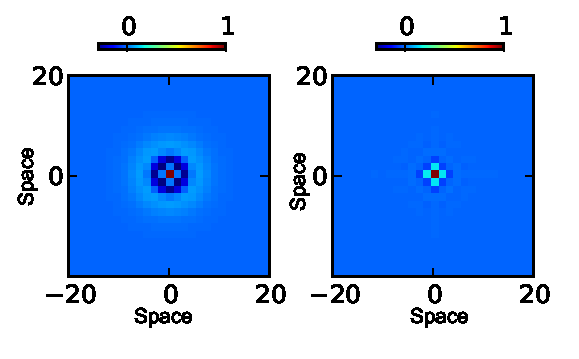
\includegraphics{./Figures/KernelWidthEstimation.pdf}
\end{center}
\caption{{\bf Estimation of Connectivity Kernel Support}. The kernel values are normalised. True  and estimated kernels are shown with solid and dotted lines respectively.}
\label{fig:KernelWidth}
\end{figure}


\bibliographystyle{plain}
\bibliography{}
\end{document}
